\section{Evaluation}

  The present section aims at evaluating on a COTS platform the benefits brought by SchIM (w.r.t. memory isolation) and to demonstrate the good behaviour of the different embedded policies. Therefore, we have integrated the SchIM IP on the PL side of a Xilinx ZCU102 development board, featuring a Xilinx Zynq UlraScale+ XCZU9EG SoC. For this work, we evaluate SchIM using synthetic benchmarks, real benchmarks issued from the San Diego Vision Benchmark Suite (SD-VBS) \cite{SD-VBS} and combinations of the two.
  
  The present section is organised as follows. Firstly, in subsection \ref{subsection:considered-architecture}, the exact SchIM configuration on the ZCU102 development board is discussed. Thereafter, a full assessment of the board capabilities with and without SchIM is provided in subsection \ref{subsec:platform-capabilities-and-performance-degradation}. In subsection \ref{subsec:internal-behaviour-of-schim}, an analysis of the SchIM module behaviour is presented. Finally, a demonstration of the memory isolation enabled by SchIM using real benchmark applications is provided.

  \subsection{Considered architecture}
    \label{subsection:considered-architecture}

  \subsection{Platform Capabilities and performance degradation}
    \label{subsec:platform-capabilities-and-performance-degradation}
    Intuitively and as discussed in \cite{PLIM20}, redirecting the traffic coming from the cores cluster to the PL side has a cost. In fact, the PL side running at a lower frequency and being further away on the System-on-Chip, one core will experience both a bigger latency and a smaller throughput. On the other hand, by redirecting the traffic to the PL side, we can achieve higher system predictability.
    
    In order to weight up the pro and the cons of these two orthogonal objectives, we have computed the throughput of one \emph{core under analysis}, here core 0 (noted $C_{0}$), for different configurations. The result of this experiment is display in Figure \ref{fig:bandwidth_comparison}. The configurations are a combination of a varying amount of cores competing (x axis) and different path between the cores cluster to the main memory (the different bars). More accurately, we consider five paths (i) all the cores target the main memory (referred to as \emph{Normal Route}), (ii) all the cores target a single HPM port, like they would in PLIM \cite{PLIM20} (referred to as \emph{PL Loop-back}), (iii) all the cores target the \schim IP configured to apply FP (referred to as \emph{SchIM FP}), (iv) all the cores target the \schim IP configured to apply TDMA (referred to as \emph{TDMA}) and (v) all the cores target the \schim IP configured to apply TS (referred to as \emph{SchIM MG}). These configurations are compared with respect to the throughput (expressed in MBps) that the core under analysis (i.e., core 0) experiences (y axis).
    
    From the Figure \ref{fig:bandwidth_comparison}, one can observe that in general, the throughput experienced by the core under analysis (i.e., $C_{0}$) is high and that, regardless of the contention level, the bandwidth remains high. As mentioned earlier, redirecting the cores traffic through the PL side has a cost. In fact, in the case with no contention (the left most bar cluster), the bandwidth experienced by $C_{0}$ when redirecting the traffic to a simple loop-back, is four times smaller than the normal route.
    Using the left most bar cluster, one can also observe the overhead introduced by having \schim on the memory loop-back. The overhead is approximatly of ?? MBps.
    While the throughput in the case of a \emph{PL loop-back} is bigger, it also falls as soon as the contention level increases.
    On the other hand, the \schim IP manages to preserve the same bandwidth, with only small interferences being observed in the most challenging scenario (the right most bar cluster). In other words, \schim guarantees isolation of the cores w.r.t. the bus usage.
     
    \begin{figure}
      \centering
      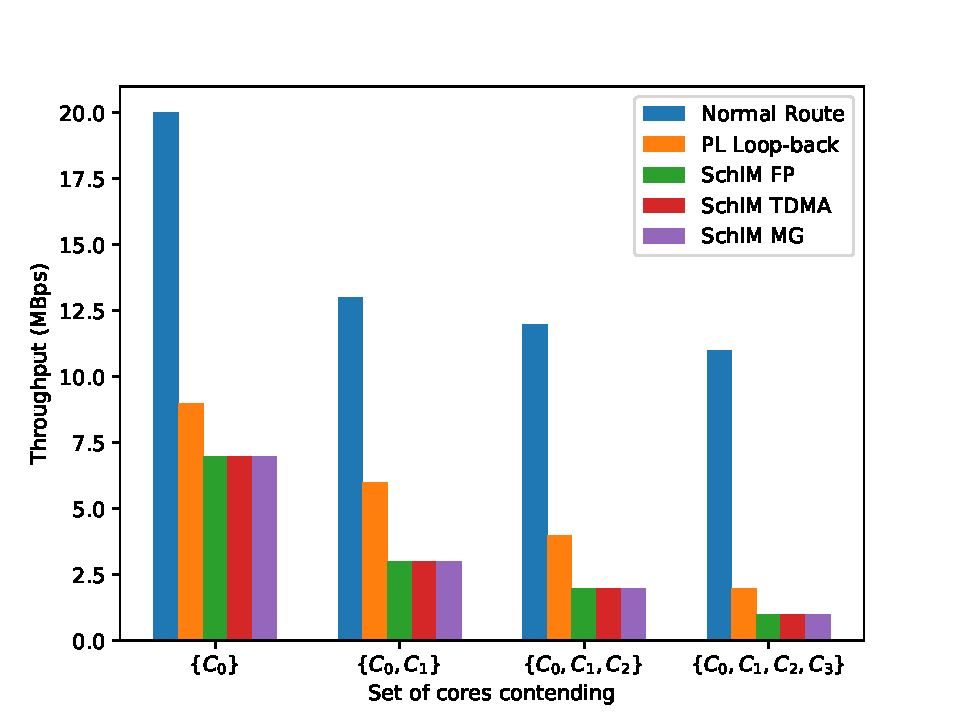
\includegraphics[scale=0.5]{images/bw_comparisons.pdf}
      \caption{Board bandwidth}
      \label{fig:bandwidth_comparison}
    \end{figure}

  \subsection{Internal Behaviour of SchIM}
    \label{subsec:internal-behaviour-of-schim}    
    As mentioned earlier, the next objective is to verify the correct behaviour of our scheduling policies at the granularity of a clock cycle by observing the inputs, the outputs and the internal signals and registers of the \schim module.
    This is made possible thanks to the \emph{Integrated Logic Analyser} (or ILA) provided by Xilinx \cite{Xilinx-ILA}. The latter IP can be directly implemented on the PL side, alongside the \schim IP, and is able to probe and signals and to store them in a local memory. For this experiment, the desired signals have been probed and captured during a window of 16384 contiguous clock cycles. Then, the information has been extracted by post-processing the data.
    To characterise the behaviour of the three different policies, the ILA has been used to collect (i) the amount of transactions being buffered in the queues at each clock cycle (subfigure 1 in Figure \ref{fig:schim_behaviour_fp}, \ref{fig:schim_behaviour_tdma}, \ref{fig:schim_behaviour_mg}), (ii) the rate at which queues receive new transactions from the cores cluster (subfigure 2 in Figure \ref{fig:schim_behaviour_fp}, \ref{fig:schim_behaviour_tdma}, \ref{fig:schim_behaviour_mg}) and (iii) the queues ID of each transaction repeated by the \schim module (subfigure 3 in Figure \ref{fig:schim_behaviour_fp}, \ref{fig:schim_behaviour_tdma}, \ref{fig:schim_behaviour_mg}).
    
    For the Fixed Priority trace snapshot displayed in Figure \ref{fig:schim_behaviour_fp}, the following strict priority ordering has been considered: $C_{0} \succ C_{1} \succ C_{2} \succ C_{3}$ where the $\succ$ operator means that the left argument has a strictly higher priority than the right argument. In this experiment, a threshold of 2 for each core has been used.
    As emphasized by the subfigure 2 of Figure \ref{fig:schim_behaviour_fp}, the FP scheduler is able to prioritize the traffic of one core at the expense of the others according to the priorities assignment. Furthermore, one can observe that the rate at which the queues receive new transactions from their associated core is proportional to the priority place in the priority ordering.
    Finally, the third subfigure of Figure \ref{fig:schim_behaviour_fp} confirms the correct behaviour of the FP policy. Thanks to the heat map, one can clearly see that the cores with the highest priority also feature the highest density of transactions at the output of \schim.
    
    The trace snapshot displayed in Figure \ref{fig:schim_behaviour_tdma} has been obtained by configuring the \schim module in TDMA mode. For the sake of clarity, a period of 512 clock cycles have been set for ech core. In addition, the threshold of each core has been set to 1.
    The subfigures 2 and 3 of Figure \ref{fig:schim_behaviour_tdma} clearly show the behaviour expected from a TDMA schedule. In fact, one can clearly see in the latter that transactions originating from one core are only being repeated out of the \schim module during a well defined time slot (here, our 512 clock cycles period). Moreover, queues are scheduled one after the other in a periodic fashion.
    In the subfigure 2 of Figure \ref{fig:schim_behaviour_tdma}, we can observe a similar pattern, with transactions arriving only during the TDMA slot associated to their queue (and indirectly core). Globally, the rate at which queues receive transactions is steady and constant. The small variations can be explained by different factors such as the coarseness of the FIQ feedback regulation and the scheduling happening on the hypervisor or OS levels.
    
       The trace snapshot for the TS policy has been obtained with the minimal inter-arrival period set to 256 clock cycles for all the cores. Sinilarly to the TDMA experiment, such period has been set arbitrarily in order to improve teh clarity of the trace snapshot displayed in Figure \ref{fig:schim_behaviour_mg}.
       Thanks to the subfigure 3 of Figure \ref{fig:schim_behaviour_mg}, we can see that under an important traffic load, the TS mode of \schim is able to shape the traffic. In the present case, it introduces a minimal time distancing between two transactions originating from a smae core.
       Roughly, the same pattern can be observed in subfigure 2 of Figure \ref{fig:schim_behaviour_mg}. However, there are two exceptions. First, one queue can receive more than one transaction. This is due to the coarseness of the FIQ feedback regulation. Secondly, some queues seem to be prioritized. This can be explained by the fact that in the TS scheduler implementation, ties between valid transactions are resolved by applying a FP policy. In this experiment, the \schim module being constantly under pressure, there are always ties between the queues and FP is always applied.
    \begin{figure}[]
      \centering
      \begin{subfigure}{0.5\textwidth}
        \centering
        % include first image
        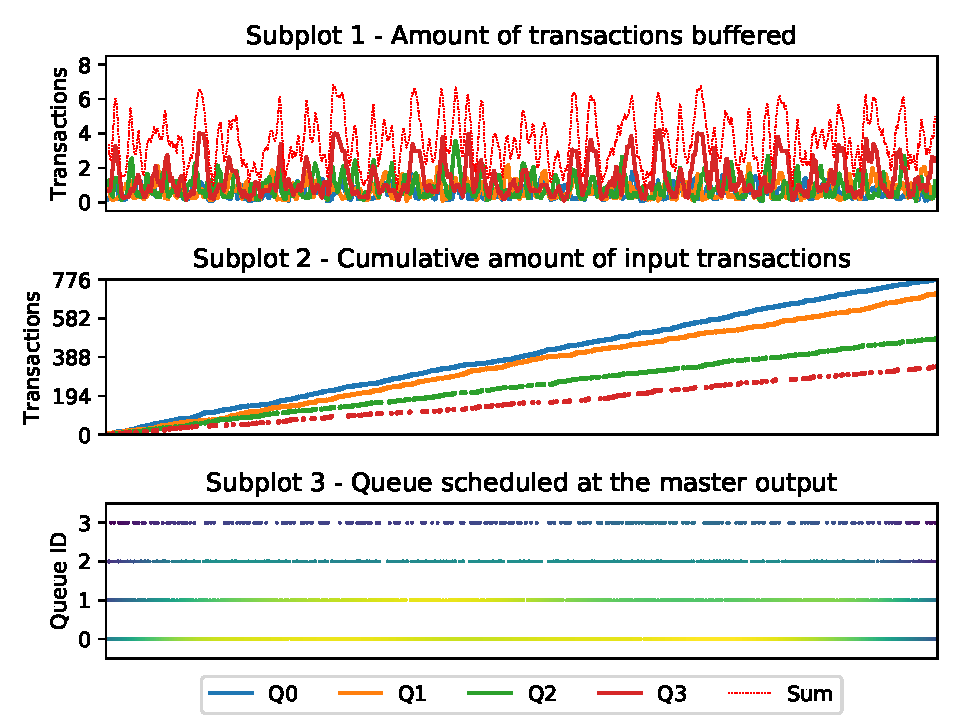
\includegraphics[scale=0.55]{images/SchIM_FP_buffering.pdf}
        \caption{FP with ordering $C_{0} \succ C_{1} \succ C_{2} \succ C_{3}$}
        \label{fig:schim_behaviour_fp}
      \end{subfigure}
      \vfill
      \begin{subfigure}{0.5\textwidth}
        \centering
        % include second image
        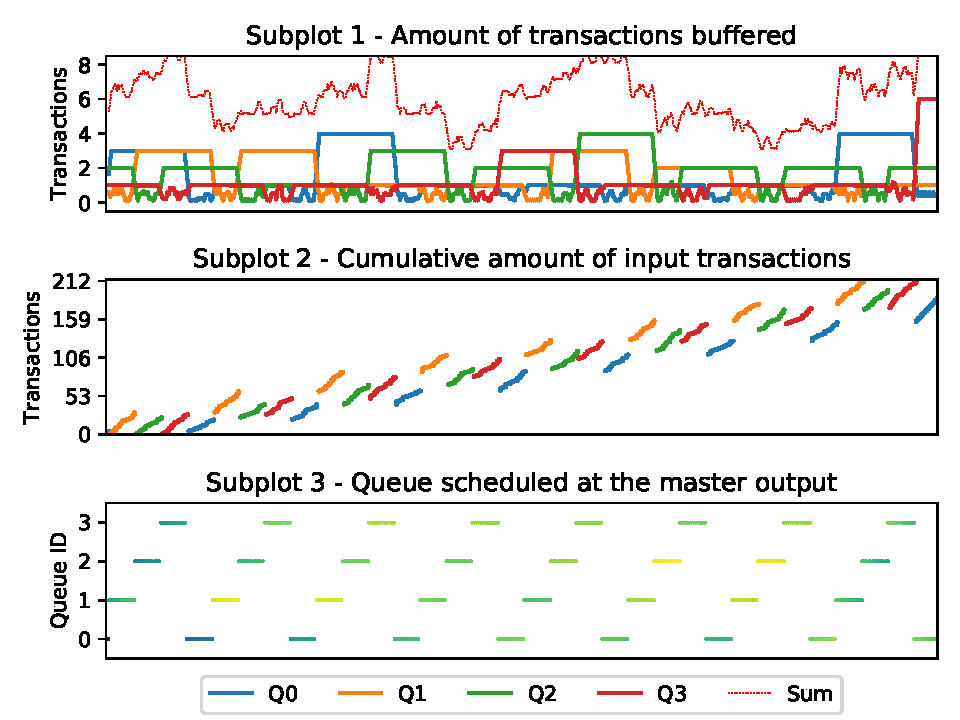
\includegraphics[scale=0.55]{images/SchIM_TDMA_buffering.pdf}
        \caption{TDMA with slots of 512 clock cycles}
        \label{fig:schim_behaviour_tdma}
      \end{subfigure}
      \vfill
      \begin{subfigure}{0.5\textwidth}
        \centering
        % include second image
        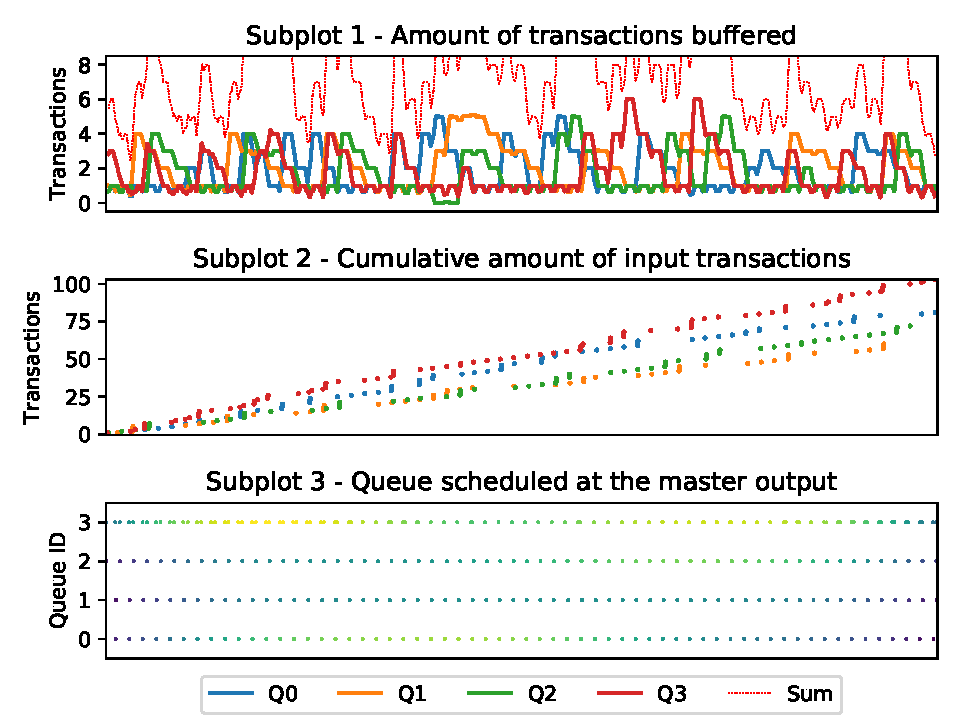
\includegraphics[scale=0.55]{images/SchIM_MG_buffering.pdf}
        \caption{TS with min. period of 256 clock cycles}
        \label{fig:schim_behaviour_mg}
      \end{subfigure}
      \caption{Trace snapshots of SchIM for FP (\ref{fig:schim_behaviour_fp}), TDMA (\ref{fig:schim_behaviour_tdma}) and TS (\ref{fig:schim_behaviour_mg})}
      \label{fig:schim_behaviour}
    \end{figure}

  \subsection{Memory Isolation}
    Here, prove that SchIM enables us to isolate the cores. We need a bunch of benchmarks competing with mem-bombs on the remaining cores. We will try:
    \begin{itemize}
      \item FP:~ The benchmark running alone with the highest priority VS. the same setup with mem-bombs
      \item TDMA:~ The benchmark running alone with all the cores having a slot of the same size VS. the same setup with mem-bombs
      \item MG:~ The benchmark running alone with all the cores having a given periodicity VS. the same setup with mem-bombs
    \end{itemize}
